\documentclass[border=10pt]{standalone}

\usepackage{tikz}
\usepackage{tikzsymbols}
\usetikzlibrary{calc,patterns,shapes.geometric}

\def\centerarc[#1](#2)(#3:#4:#5){\draw[#1] ($(#2)+({#5*cos(#3)},{#5*sin(#3)})$) arc (#3:#4:#5);}

\begin{document}
	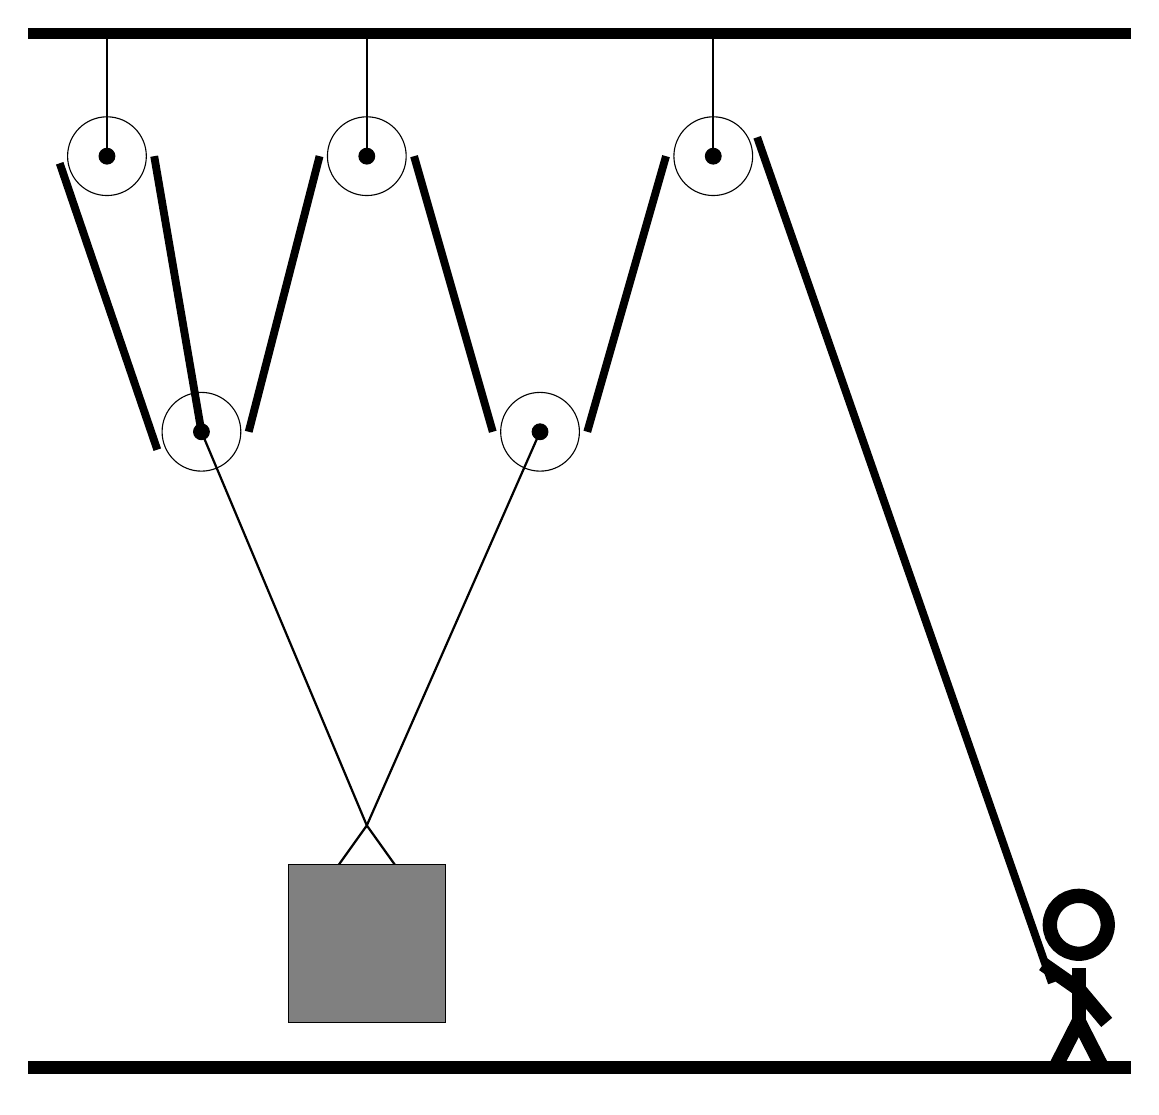
\begin{tikzpicture}
		%%%%% START %%%%%
		\draw[fill=black] (-2, 10) rectangle (12, 10.125);
		
		\draw (-1, 8.5) circle (0.5);
		\draw[fill=black] (-1, 8.5) circle (0.1);
		\draw[thick] (-1, 8.5) -- (-1, 10);
		
		\draw (2.3, 8.5) circle (0.5);
		\draw[fill=black] (2.3, 8.5) circle (0.1);
		\draw[thick] (2.3, 8.5) -- (2.3, 10);
		
		\draw (6.7, 8.5) circle (0.5);
		\draw[fill=black] (6.7, 8.5) circle (0.1);
		\draw[thick] (6.7, 8.5) -- (6.7, 10);
		
		\draw (0.2, 5) circle (0.5);
		\draw[fill=black] (0.2, 5) circle (0.1);
		
		\draw (4.5, 5) circle (0.5);
		\draw[fill=black] (4.5, 5) circle (0.1);
		
		\draw[thick] (0.2, 5) -- (2.3, 0)  -- (4.5, 5);
		\draw[thick]  (1.8, -0.7) -- (2.3, 0) -- (2.8, -0.7);
		\draw[fill=black!50] (1.3, -0.5) rectangle (3.3, -2.5);
		
		\draw[line width=1mm] (0.2, 5) -- (-0.4, 8.5);
		\centerarc[line width=1mm](-1, 8.5)(0:200:0.6);
		\draw[line width=1mm] (-1.6, 8.41) -- (-0.361, 4.772);
		\centerarc[line width=1mm](0.2, 5)(200:360:0.6);
		\draw[line width=1mm](0.8, 5) -- (1.7, 8.5);
		\centerarc[line width=1mm](2.3, 8.5)(0:180:0.6);
		\draw[line width=1mm] (2.9, 8.5) -- (3.9, 5);
		\centerarc[line width=1mm](4.5, 5)(180:360:0.6);
		\draw[line width=1mm] (5.1, 5) -- (6.1, 8.5);
		\centerarc[line width=1mm](6.7, 8.5)(20:180:0.6);
		\draw[line width=1mm](7.258, 8.74)  -- (11, -2);
		
		\node at (11.3, -2) {\Strichmaxerl[10][-35][-50]};
		
		\draw[fill=black] (-2, -3) rectangle (12, -3.15);
		%%%%% END %%%%%
	\end{tikzpicture}
\end{document}